\documentclass[11pt, ngermanm, titlepage]{article}
\usepackage[ngerman]{babel}
\usepackage{fancyhdr}
\usepackage{multicol}
\usepackage{a4wide}
\usepackage{tabu, tabularx}
\usepackage{graphicx}
\usepackage{fontspec}

\setmainfont{Arial}
\newfontfamily\jubilo[Ligatures=TeX]{Monotype Corsiva}

\setlength{\columnsep}{1cm}
\setlength{\columnwidth}{10cm}
\setlength{\extrarowheight}{15pt}

\begin{document}
	\pagenumbering{gobble}
	\begin{titlepage}
	\centering
	\includegraphics[width=0.8\textwidth]{img/cvlogo.png}\par\vspace{2cm}
	
	{\scshape\Large Sommerkonzert\par}
	\vspace{1.5cm}
	{\fontsize{50}{60}\bfseries\jubilo Sommerkonzerttitel\par}
	\vspace{1.5cm}
	{\scshape\LARGE Camerata Vocale München\par}
	\vspace{1cm}
	{\Large\itshape Leitung: Clayton Bowman\par}
	\vfill
	21.07.2019\par
	Erlöserkirche München
	
	\vfill
	
	% Bottom of the page
	{\scriptsize Mitglied im\par}
	\includegraphics[width=0.25\textwidth]{img/vdkc_logo_klein.jpg}\par\vspace{2cm}


	\end{titlepage}

	\pagebreak

	
	\section*{Programm}
	\begin{tabularx} \textwidth {lX}
		Claude Debussy (1862 - 1918) & Trois Chansons: \newline I. Dieu! qu'il la fait bon regarder! \newline II. Quant j'ai ouy le tabourin \newline III. Yver, vous n'estes qu'un villain;
		\\
		Edward Elgar (1857 - 1934) & Two Choral Songs, Op. 71: \newline 1. The Shower \newline 2. The Fountain
		\\
 		 & Death on the Hills, Op. 72
 		\\
 		 & Two Choral Songs, Op. 73: \newline 1. Love's Tempest \newline 2. Serenade
		\\
		Igor Stravinsky (1882 - 1971) & Mass: \newline Kyrie \newline Gloria \newline Credo \newline Sanctus \newline Agnus Dei
	\end{tabularx}
	\pagebreak

	\begin{multicols}{2}
	\section*{Andreas Hammerschmidt}
	\paragraph{(geboren 1611 oder 1612 in Brüx, Böhmen; gestorben 1675 in Zittau)\newline}
	Der deutsche Organist und Komponist Andreas Hammerschmidt (auch „-schmied“ oder „-schmiedt“) floh mit seiner Familie vor der forcierten Rekatholisierung in Böhmen und gelangte so nach Freiberg im Kurfürstentum Sachsen, wo er vermutlich seine musikalische Ausbildung erhielt. Nach zwei vorausgehenden Organistenstellen ließ er sich schließlich 1639 als Organist in der damals reichen Stadt Zittau nieder, wirkte dort bis zu seinem Lebensende und gelangte zu gesellschaftlichem Ansehen und überdurchschnittlichem materiellem Wohlstand.
	
	Als Komponist des Frühen bis Mittleren Barock ist er in die Gruppe der evangelisch-lutherischen Kirchenkomponisten wie Heinrich Schütz und Johann Sebastian Bach einzuordnen. Sein kompositorisches Schaffen umfasst unter anderem Lieder, Kantaten, Motetten und Instrumental- wie auch Vokalkompositionen. Im Jahre 1757 vernichtete der große Stadtbrand in Zittau leider einen Großteil der Quellen über Hammerschmidt.
	
	\textit{Quelle: Deutsch- und englischsprachige Wikipedia}

	
	\section*{Thomas Weelkes}
	\paragraph{(geboren 1576 in Elsted, West Sussex; gestorben 1623 in London)\newline}
	Der englische Komponist Thomas Weelkes wurde 1598 zum Organisten des Winchester College ernannt und wechselte 1601 in die Kathedrale von Chichester. Dort wurde er jedoch später entlassen, da er an der Orgel getrunken hatte und während des Gottesdienstes schmutzige Worte benutzte. Weelkes, ein Meister der Wortmalerei, war als Madrigalist bekannt, dessen zweiter Band (1600 veröffentlicht) eine der wichtigsten Sammlungen in der englischen Madrigal-Tradition ist.

	\textit{Quellen: emmanuelmusic.com,	Wikipedia}
	
	
	\section*{Francis Poulenc}
	\paragraph{(geboren 1899, Paris; gestorben 1963, ebenda)\newline}
	Francis Jean Marcel Poulenc wuchs in einem musikalischen Haushalt auf und erhielt ersten Klavierunterricht durch seine Mutter. Nach weiterer Ausbildung als Pianist blieb das Klavier zunächst zentral und dominiert seine frühen Werke. Nicht nur Stravinsky, Chevalier und das französische Vaudeville beeinflussten ihn, sondern auch der Freund und Mentor Erik Satie, der sich dem damaligen französischen musikalischen Mainstream entzog, sowie seine Mitgliedschaft im Komponistenzirkel „Les Six“, der den Impressionismus zugunsten einer größeren Einfachheit und Klarheit ablehnte. So stand Poulenc beispielsweise Ravels musikalischen Ansichten kritisch gegenüber, wenngleich er ihn als Person sehr respektierte. Poulencs Bewusstsein für seine Insuffizienz in Bezug auf das technische Niveau seiner weitestgehend autodidaktisch erworbenen kompositorischen Fertigkeiten bewog ihn später zu Unterricht bei Charles Koechlin. Nach ab den 1920er Jahren – auch als Pianist – eintretendem internationalem Erfolg führten 1936 der Unfalltod eines Freundes und der Besuch des Wallfahrtsortes Rocamadour dazu, dass sich der Komponist intensiv auf den katholischen Glauben zurückbesann, mit der Komposition geistlicher Werke begann und eine stilistisch ernstere Komponente entwickelte. Die letzterer entspringenden Werke erhielten erst in den 1950er Jahren größere Anerkennung.
	
	Im Privatleben stellten der (während der Nazibesetzung auch politische) Umgang mit seiner Homosexualität sowie wiederkehrende, seine Schaffenskraft beeinflussende Depressionen Herausforderungen dar.
	
	Poulenc selbst verstand seinen Schaffensschwerpunkt in der Komposition von Opern. Kritiker sehen insbesondere die Dualität seiner stilistischen Pole: leichtherzig bis pietätlos versus ernsthaft-gewichtig. Das Gesamtwerk gilt als weitestgehend diatonisch und melodiezentriert und umfasst Bühnenwerke, Filmmusik, Geistliche Werke, weltliche Chorwerke, Kammermusik, zahlreiche Lieder sowie Klavier- und Orchesterwerke.
	
	\textit{Quelle: Deutsch- und englischsprachige Wikipedia}
	
	\section*{Michael Praetorius}
	\paragraph{(geboren 1571 in Creuzburg bei Eisenach; gestorben 1621 in Wolfenbüttel)\newline}
	Michael Praetorius, eigentlich Michael Schulteis, war ein deutscher Komponist, Organist, Hofkapellmeister und Gelehrter im Übergang von der Renaissance- zur Barockzeit. Sein Vater war Pfarrer, der in Wittenberg bei Martin Luther studiert hatte. Auch die beiden älteren Brüder wurden Pfarrer, und so schrieb sich auch Michael Praetorius schon mit 11 Jahren an der Universität in Frankfurt/Oder für Theologie ein. Als der Vater und die Brüder starben, war niemand mehr da, der den 16-jährigen finanziell unterstützen konnte. Er wechselte auf die Orgelbank, um seinen Lebensunterhalt zu verdienen. Auch ohne geregelte musikalische Ausbildung erwarb er sich schnell einen überregionalen Ruf. So kam er an den Hof des musikliebenden Herzogs Heinrich Julius zu Braunschweig. 
	
	Am Hof in Wolfenbüttel und Gröningen stieg er zum Hofkomponisten auf und entfaltete in kurzer Zeit eine ungeheuer fruchtbare Nebentätigkeit als Komponist und Herausgeber. Er war ein glühender Anhänger der aufregenden musikalischen Neuerungen aus Italien am Übergang von der Renaissance zum Barock. Leider konnte er nie selbst nach Italien reisen, aber durch Kompositionen, Aufführungen und Veröffentlichungen wurde er zum Herold der Neuen Musik in Deutschland. Praetorius starb am 15. Februar 1621 und wurde unter der Orgelempore der Hauptkirche Beatae Mariae Virginis in Wolfenbüttel beigesetzt.
	
	\textit{Quelle: mh-koeln.de/cck}
	
	\section*{Randall Thompson}
	\paragraph{(geboren 1899 in New York City; gestorben 1984 in Boston) \newline}
	Randall Thompson war ein US-amerikanischer Komponist und Musikpädagoge, der vor allem für seine Chorwerke bekannt wurde. Er studierte an der Harvard University und am American Conservatory in Rom. 1927 wurde er Professor für Musik, Organist und Chorleiter am Wellesley College. Später unterrichtete er an der Harvard University, leitete verschiedene Madrigalchöre und den New Yorker Juilliard Choir und wurde Professor an der Berkeley University, der University of Virginia und der Princeton University. Seine Studie College Music (1935) bewirkte eine grundlegende Reform der universitären Musikausbildung in den USA. Thompson komponierte drei Sinfonien, zwei Opern, weitere sinfonische Werke und Kammermusik. Populär wurden jedoch vor allem seine Chorwerke.
	
	\textit{Quelle: Wikipedia}
	\vfill
	\pagebreak
	
	\section*{Camerata Vocale München}
	Die Camerata Vocale München gründete sich 2016 auf Initiative von Clayton Bowman zunächst als Projektchor mit Sängerinnen und Sängern aus München und Heidelberg.
	
	Als erstes Projekt gestaltete die Camerata am Palmsonntag 2016 einen Motettengottesdienstes mit Bachs „Jesu, meine Freude“ in der ältesten evangelischen Kirche Münchens, der St. Paulus-Kirche im Stadtteil Perlach, in welcher bis heute regelmäßig Konzerte des Chores stattfinden. Es folgten in den Jahren 2016 und 2017 weitere Aufführungen in München und Mannheim.
	
	Seit Sommer 2017 besteht die Camerata Vocale als ambitionierter Münchner Kammerchor mit regelmäßiger Probenarbeit und zählt inzwischen über 20 Mitglieder. Nach ihrem Debütkonzert im Januar 2018 mit Werken u.a. von Reger, Brahms und Vaughan Williams wirkte die Camerata an einer Produktion der Hochschule für Musik und Theater München mit, in deren Rahmen die Barockoper La Dafne von Marco da Gagliano im Rahmen der Barocktage 2018 zur Aufführung gebracht wurde. Die Konzertsaison beschloss der Chor mit zwei Auftritten in St. Paulus in Perlach sowie St. Leonhard in Nußdorf am Inn im Juli 2018, bei denen jeweils anspruchsvolle Vokalmusik aus der englischen Chortradition erklang.  Bei einem festlichen Adventskonzert brachte die Camerata im Dezember 2018 u.a. Werke von Poulenc, Praetorius, Thompson und Howells zur Aufführung. Mit diesem Programm debütierte der Chor zugleich im Rahmen der Foyer-Konzerte der TH Rosenheim.
	
	Neben ihrer Konzerttätigkeit übernimmt die Camerata Vocale in regelmäßigen Abständen die musikalische Gestaltung von  Gottesdiensten in der KHG der LMU und der Evangelischen St. Paulus-Gemeinde in Perlach. Die hohe Qualität, die der junge Chor in kurzer Zeit erreicht hat, bezeugt unter anderem die Aufnahme in den Verband Deutscher Konzertchöre e.V..
	
	\paragraph{Besetzung\newline}
	\begin{tabularx}\textwidth {lX}
	Sopran I & Sina Dresp \newline Susanne Haas \newline Cosima Stocker \\
	Sopran II & Kathrin Sollfrank \newline Ruth Stärcke \\
	Alt I &  Anna Hausner \newline Esther Stärcke \newline Nora Reinbold \\
	Alt II & Hannah Schade \newline Salome Schuldt \\
	Tenor I & Philipp Hummel \newline Andru \\
	Tenor II & Julius Kiendl \newline Benedikt Linder \\
	Bass I & Konrad Brückel \newline Tobias Gumpp \newline Freddy Zumegen \\
	Bass II & Joe Kübler \newline Andi Scharfstein
	\end{tabularx}
	\pagebreak

	\section*{Clayton Bowman}
	Clayton Bowman, geboren in Pittsburgh (USA), erhielt seinen ersten Klavierunterricht im Alter von 7 Jahren und wurde schon in jungen Jahren an die Chormusik herangeführt. Er sang in mehreren Auswahlchören und durfte bereits im Alter von 13 Jahren als Knaben-Solist sein Operndebüt in Benjamin Brittens "`Noye's Fludde"' mit dem Hartford Symphony Orchestra feiern.
	
	Erste Dirigiererfahrung sammelte Bowman während seiner Schulzeit. Bereits mit 14 Jahren leitete er als "`Student Conductor"' das symphonische Blasensemble an der Tolland Middle School und nahm im Jahr 2000 an einem Dirigiermeisterkurs an der University of South Carolina teil. Ab 2001 studierte er an der University of Connecticut Gesang und Musikwissenschaft mit Schwerpunkt Ensemblearbeit. Dieses Studium führte ihn schließlich nach Deutschland, wo er von 2004 bis 2008 Dirigieren bei Prof. Georg Grün, Klaus Thielitz und Wolfgang Seeliger an der Hochschule für Musik und Darstellende Kunst Mannheim studierte. Parallel dazu war Bowman lange Zeit Sänger und Dirigent zahlreicher Ensembles der Rhein-Neckar-Region.
	
	Als musikalischer Assistent beim Konzert Darmstadt und stellvertretender Dirigent des Universitätsorchesters Mannheim sammelte der junge Dirigent Erfahrung mit der Einstudierung großer Werke, wie beispielsweise Johann Sebastian Bachs "`Matthäuspassion"' und hatte zeitgleich die Leitung des Kammerchors Altrip, des Prot. Kirchenchors Mutterstadt und der Frauenchöre der Prot. Gemeinde in Dannstadt inne. Zusätzlich zu seinen Tätigkeiten als Dirigent, musizierte er häufig zusammen mit der Heidelberger Kantorei und der Hochschule für Kirchenmusik Heidelberg als Chorsänger und Solist. Darüber hinaus sang er regelmäßig im Kammerchor Saarbrücken, im Chor der Staatsphilharmonie Rheinland-Pfalz und gastierte gelegentlich als Chorist auf der Bühne des Nationaltheaters Mannheim und an der Oper Frankfurt.
	 
	Besonders aber mit dem Anglistenchor, einem der beiden Kammerchöre der Universität Heidelberg, hat sich Bowman einen Namen gemacht und eine große Leidenschaft für anspruchsvolle A-cappella-Musik entwickelt. Der Chor wirkte unter seiner Leitung vielfach im Ausland und arbeitete mit weltbekannten Chören wie dem Choir of Gonville und dem Caius College Cambridge zusammen.
	 
	Seit 2016 in München, leitet Bowman neben der vom ihm gegründeten Camerata Vocale München auch den Großen Chor des Akademischen Gesangvereins (AGV) und den Chor TonArt Sauerlach-Holzkirchen.
	\vfill
	\pagebreak
	
	\section*{Texte}
	
	\paragraph{Trois Chansons (1898 - 1908)\newline}
	I. Dieu qu'il la fait bon regarder!\newline
	La gracieuse bon et belle!\newline
	Pour les grands bien que sont en elle.\newline
	Chacun est pres de la loüer.\newline
	Qui se pourroit d'elle lasser?\newline
	Tousjours sa beauté renouvelle.\newline
	Dieu qu'il la bon regarder.\newline
	La gracieuse bonne et belle!\newline
	Par de ça, ne de là, la mer.\newline
	Ne scay dame ne damoiselle\newline
	Qui soit en tous bien parfais telle.\newline
	C'est un songe que d'i penser:\newline
	Dieu qu'il la fait bon regarder!\newline
	Dieu! qu'il la fait bon regarder!\newline
		
	II. Quant j'ai ouy le tabourin\newline
	Sonner pour s'en aller au may\newline
	En mon lit n'en ay fait effray\newline
	Ne levé mon chief du coissin\newline
	En disant: il est trop matin\newline
	Ung peu je me rendormirai:\newline
	Quant j'ai ouy le tabourin\newline
	Sonner pour s'en aller au may.\newline
	Jeunes gens partent leur butin:\newline
	De non chaloir m'accointeray\newline
	A lui je m'abutineray\newline
	Trouvé l'ay plus prouchain voisin;\newline
	Quant j'ai ouy le tabourin\newline
	Sonner pour s'en aller au may.\newline
	En mon lit n'en ay fait effray\newline
	Ne levé mon chief du coissin.\newline
	
	III. Yver, vous n'estes qu'un villain;\newline
	Esté est plaisant et gentil\newline
	En témoing de may et d'avril\newline
	Qui l'accompaignent soir et main.\newline
	Esté revet champs, bois et fleurs\newline
	De sa livrée de verdure\newline
	Et de maintes autres couleurs\newline
	Par l'ordonnance de nature.\newline
	Mais vous Yver, trop estes plein\newline
	De nège, vert, pluye et grézil.\newline
	On vous deust banir en évil.\newline
	Sans point flater je parle plein,\newline
	Yver, vous n'estes qu'un villain.\newline
	
	\paragraph{Two Choral Songs, Op. 71 (1914)\newline}
	\textbf{1. The Shower}\newline
	Cloud, if as thou dost melt, and with thy train\newline
	Of drops make soft the Earth, my eyes could weep\newline
	O'er my hard heart, that's bound up and asleep;\newline
	Perhaps at last,\newline
	Some such showers past\newline
	My God would give a sunshine after rain.\newline
	
	\textbf{2. The Fountain}\newline
	The unthrift sun shot vital gold,\newline
	A thousand, thousand pieces;\newline
	And heav'n its azure did unfold\newline
	Chequer'd with snowy fleeces;\newline
	The air was all in spice,\newline
	And ev'ry bush\newline
	A garland wore:\newline
	Thus fed my eyes,\newline
	But all the earth lay hush,\newline
	Only a little fountain lent\newline
	Some use for ears,\newline
	And on the dumb shades language spent,\newline
	The music of her tears.\newline
	
	\paragraph{Death on the Hills, Op. 72 (1914)\newline}
	Why o'er the dark'ning hill-slopes\newline
	Do dusky shadows creep?\newline
	Because the wind blows keenly there,\newline
	Or rainstorms lash and leap?\newline
	
	No wind blows chill upon them,\newline
	Nor are they lash'd by rain:\newline
	'Tis Death who rides across the hills\newline
	With all his shadowy train.\newline
	
	The old bring up the cortege,\newline
	In front the young folk ride,\newline
	And on Death's saddle in a row\newline
	The babes sit side by side.\newline
	
	The young folk lift their voices,\newline
	The old folk plead with Death:\newline
	"O let us take the village-road,\newline
	Or by the brook draw breath.\newline
	
	"There let the old drink water,\newline
	There let the young folk play,\newline
	And let the little children\newline
	Run and pluck the blossoms gay."\newline
	
	[Death speaks]\newline
	"I must not pass the village\newline
	Nor halt beside the rill,\newline
	For there the wives and mothers all\newline
	Their buckets take to fill.\newline
	
	"The wife might see her husband,\newline
	The mother see her son;\newline
	So close they'd cling - their claspings\newline
	Could never be undone."\newline
	
	\paragraph{Two Choral Songs, op. 73 (1914)\newline}
	\textbf{1. Love’s Tempest}\newline
	Silent lay the sapphire ocean,\newline
	Till a tempest came to wake\newline
	All its roaring, seething billows\newline
	That upon earth's ramparts break.\newline
	
	Quiet was my heart within me\newline,
	Till your image, suddenly\newline
	Rising there, awoke a tumult\newline
	Wilder than the storm at sea.\newline
	
	\textbf{2. Serenade}\newline
	Dreams all too brief,\newline
	Dreams without grief,\newline
	Once they are broken, come not again.\newline
	
	Across the sky the dark clouds sweep,\newline
	And all is dark and drear above:\newline
	The bare trees toss their arms and weep,\newline
	Rest on, and do not wake, dear Love.\newline
	
	Since glad dreams haunt your slumbers deep,\newline
	Why should you scatter them in vain?\newline
	
	Happy is he, when Autumn falls,\newline
	Who feels the dream-kiss of the Spring;\newline
	And happy he in prison walls\newline
	Who dreams of freedom's rescuing;\newline
	
	But woe to him who vainly calls\newline
	Through sleepless nights for ease from pain?\newline
	
	\paragraph{Mass (1944-1948)\newline}
	\textbf{Kyrie}\newline
	Kyrie, eleison.\newline
	Christe, eleison.\newline
	Kyrie, eleison.\newline
	
	\textbf{Gloria}\newline
	Gloria in excelsis Deo,\newline
	et in terra pax hominibus bonae voluntatis.\newline
	Laudamus te. Benedicimus te.\newline
	Adoramus te. Glorificamus te.\newline
	Gratias agimus tibi propter magnam gloriam tuam.\newline
	Domine Deus, Rex coelestis,\newline
	Deus Pater omnipotens,\newline
	Domine Fili unigenite, Iesu Christe;\newline
	Domine Deus, Agnus Dei, Filius Patris:\newline
	qui tollis peccata mundi,\newline
	miserere nobis;\newline
	qui tollis peccata mundi,\newline
	suscipe deprecationem nostram;\newline
	qui sedes ad dexteram Patris,\newline
	miserere nobis.\newline
	Quoniam tu solus Sanctus,\newline
	tu colus Dominus,\newline
	tu solus Altissimus, Iesu Christe.\newline
	Cum Sancto Spiritu in gloria Dei Patris.\newline
	Amen.\newline
	
	\textbf{Credo}\newline
	
	Credo in unum Deum, Patrem omnipotentem, factorem coeli et terrae, visibilium omnium, et invisibilium.\newline
	Et in unum Dominum Iesum Christum Filium Dei unigenitum.\newline
	Et ex Patre natum ante omnia saecula.\newline
	Deum de Deo, lumen de lumine, Deum verum de Deo vero.\newline
	Genitum, non factum, consubstantialem Patri: per quem onmia facta sunt.\newline
	Qui propter nos homines et propter nostram salutem descendit de coelis.\newline
	Et incarnatus est de Spiritu Sancto ex Maria Virgine:\newline
	et homo factus est.\newline
	Crucifixus etiam pro nobis: sub Pontio Pilato passus, et sepultus est.\newline
	Et resurrexit tertia die, secundum Scripturas.\newline
	Et ascendit in coelum: sedet ad dexteram Patris.\newline
	Et iterum venturus est cum gloria judicare vivos et mortuos:\newline
	cujus regni non erit finis.\newline
	Et in Spiritum Sanctum, Dominum et vivificantem:\newline
	qui ex Patre Filioque procedit.\newline
	Qui cum Patre et Filio simul adoratur et conglorificatur:\newline
	qui locutus est per Prophetas.\newline
	Et unam sanctam catholicam et apostlicam Ecclesiam.\newline
	Confiteor unum baptisma in remissionem peccatorum.\newline
	Et exspecto resurrectionem mortuorum.\newline
	Et vitam venturi saeculi. Amen.\newline
	
	\textbf{Sanctus}\newline
	Sanctus, Sanctus, Sanctus Dominus Deus Sabaoth:\newline
	Pleni sunt caeli et terra gloria tua.\newline
	Hosanna in excelsis.\newline
	Benedictus quit venit in nomine Domini:\newline
	Hosanna in excelsis.\newline
	
	\textbf{Agnus Dei}\newline
	Agnus Dei, qui tollis peccata mundi, miserere nobis.\newline
	Agnus Dei, qui tollis peccata mundi, dona nobis pacem.\newline
		
	\end{multicols}
	
	\pagebreak
	\centering
	\begin{figure}
		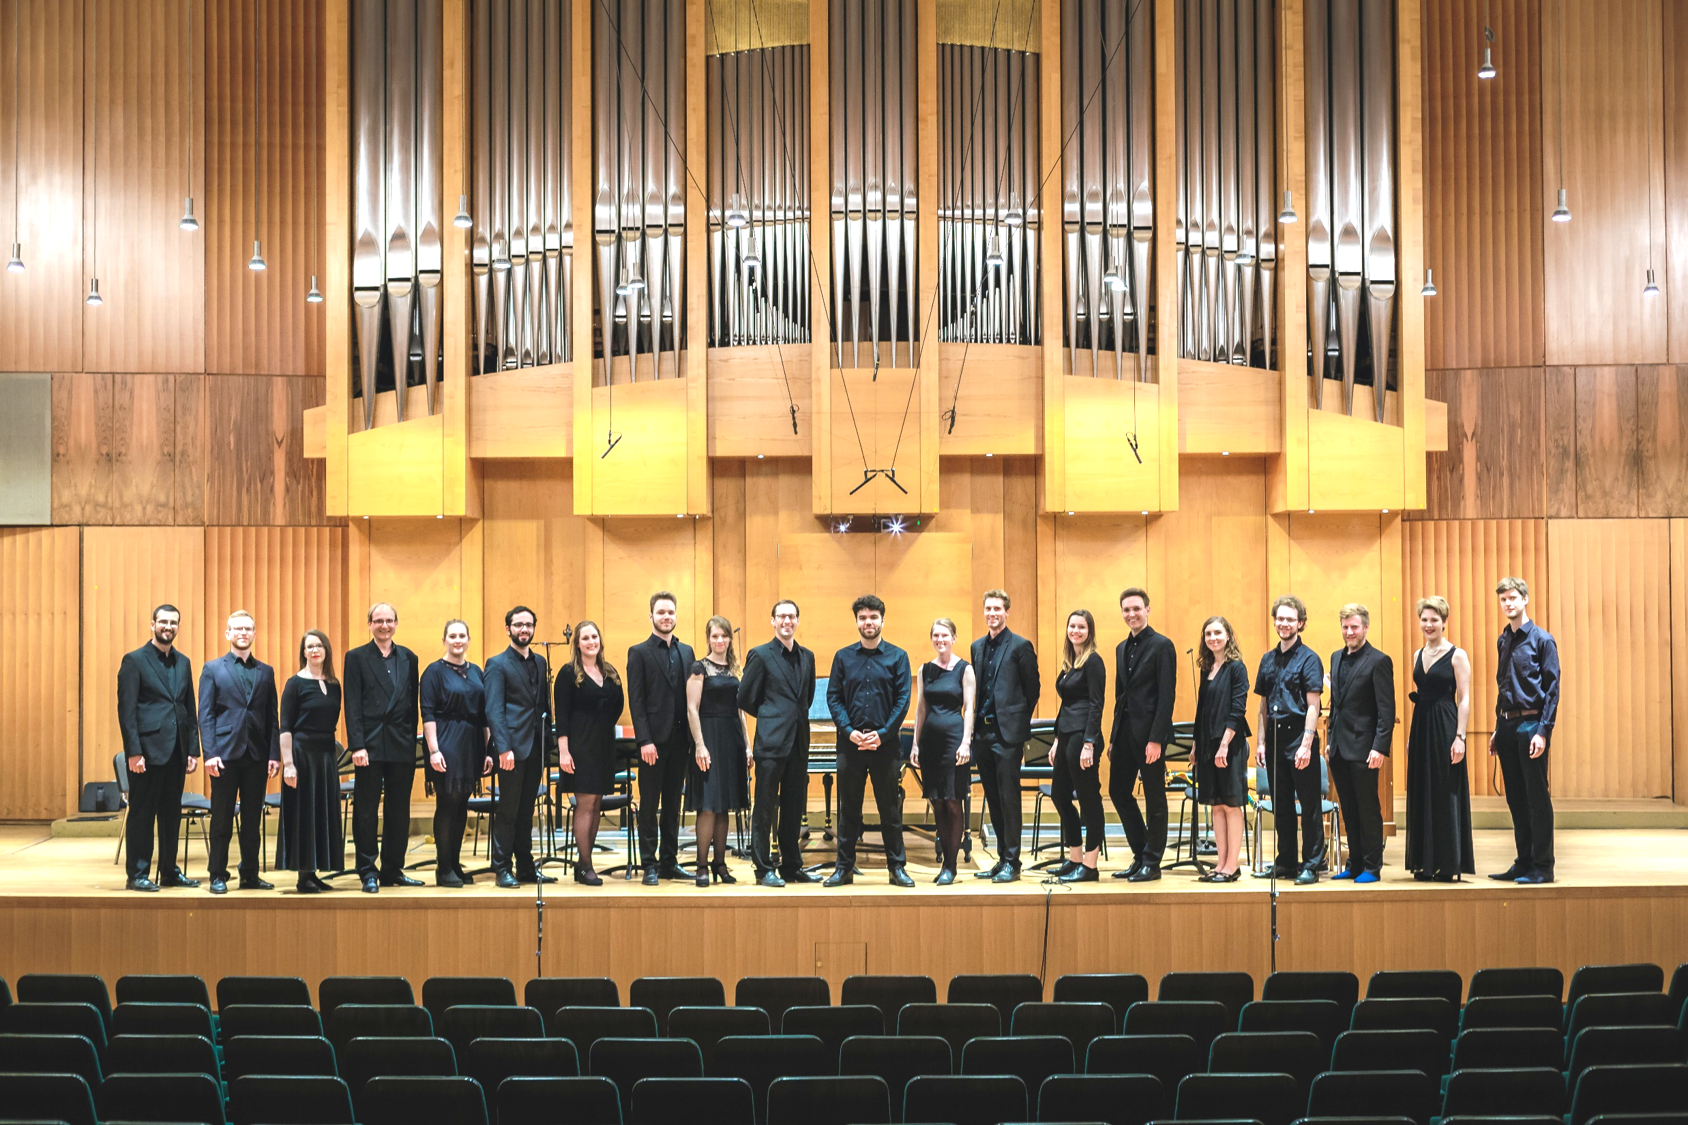
\includegraphics[width=\textwidth]{img/chorfoto_heller.png}
		\tiny{Foto: Chris Regel}
	\end{figure}
	\par\vspace{2cm}
	
	{\scshape\large Wir freuen uns sehr über Ihre Spende am Ende des Konzerts.\par
	Durch Ihre Unterstützung können wir unter anderem Programmhefte drucken oder Noten erwerben.\par}
	\vspace{1.5cm}
	{\scshape\Large Vielen Dank\par}
	\vfill
	{\small Impressum\par
		{\large Camerata Vocale München\par}
	Leitung: Clayton Bowman\par
	Kontakt: info@cameratavocale-muenchen.de\par
	www.cameratavocale-muenchen.de\par
	www.facebook.com/CVMuenchen\par
	Texte und Gestaltung: Cosima Stocker, Denise Dudek, Benedikt Linder}
	

\end{document}